\documentclass[10pt]{article}
%----------Packages----------
\usepackage[utf8]{inputenc}
\usepackage{amsmath}
\usepackage{amssymb}
\usepackage{multicol}
\usepackage[landscape, total={10.8in,8in}]{geometry}
\usepackage{blindtext}
\usepackage{graphicx}
\usepackage{siunitx}
\usepackage[shortlabels]{enumitem}
\usepackage{steinmetz}
%----------Page formatting----------
\pagenumbering{gobble}
\parindent=0pt
%----------Complex Numbers----------
\newcommand{\bv}{\boldsymbol}
\newcommand{\V}{\bv V}
\newcommand{\I}{\bv I}
\newcommand{\Z}{\bv Z}
\renewcommand{\S}{\bv S}
\renewcommand{\Re}[1]{\mathrm{Re}\sqb{#1}}
\newcommand{\conj}{^*}
\newcommand{\norm}[1]{\left\lvert #1 \right\rvert}

%----------Brackets----------
\newcommand{\lrb}[1]{\left(#1\right)}
\newcommand{\sqb}[1]{\left[#1\right]}

%----------Differentiation----------
\renewcommand{\d}{\,\mathrm{d}}
\newcommand{\dv}[2]{\frac{\mathrm{d} #1}{\mathrm{d} #2}}
\newcommand{\ddv}[2]{\frac{\mathrm{d}^2 #1}{\mathrm{d} #2^2}}

%----------Headings----------
\newcommand\sectionheading[1]{\begin{center}\large{\textbf{#1}}\end{center}\normalsize}
% \newcommand\heading[1]{\smallskip\textbf{#1}\smallskip}
\newcommand\heading[1]{\textbf{#1}}

%----------Info----------
\newcommand*{\course}{ELEC 204} 

%----------Document Begins Here----------
\begin{document}

\begin{center}
    \huge{\textbf{\course \ Formula Sheet}}
\end{center}

\begin{multicols*}{3}

\sectionheading{Basics}
\heading{Current, Voltage, Power}
\[e=\SI{1.602e-19}{\coulomb}\]
\[I=\dv qt\qquad V=\dv Wq\qquad P=VI\]
\heading{Resistors}
\[R=\rho\frac lA\]
\[V=IR\qquad P=I^2R\]
\begin{align*}
    R&=R_1+R_2+\cdots+R_n\tag{series} \\
    \frac 1R&=\frac 1{R_1}+\frac 1{R_2}+\cdots+\frac 1{R_n}\tag{parallel}
\end{align*}

\heading{KCL}
\[\sum I_{in}=\sum I_{out}\]

\heading{KVL}
\[\sum_{loop}\Delta V=0\]

\heading{Current-Voltage Division}
\begin{align*}
    I_1&=I_2 &V_1=\frac{R_1}{R_1+R_2}V \tag{series} \\
    V_1&=V_2 &I_1=\frac{R_2}{R_1+R_2}V \tag{parallel} 
\end{align*}

\heading{Wye-Delta}

$\Delta\to\mathrm Y$:
\[R_1=\frac{R_bR_c}{R_a+R_b+R_c}\]
$\mathrm Y\to\Delta$:
\[R_a=\frac{R_1R_2+R_2R_3+R_3R_1}{R_1}\]

\sectionheading{Circuit Analysis}

\heading{Nodal Analysis}
\begin{enumerate}[topsep=0pt,noitemsep]
    \item Set reference node voltage to $0$.
    \item Assign variable voltages to other nodes.
    \item Write KCL at all unknown nodes, then solve. 
    \item Use supernode if necessary.
\end{enumerate}

\heading{Mesh Analysis}
\begin{enumerate}[topsep=0pt,noitemsep]
    \item Assign loop currents.
    \item Write KVL for each loop, then solve. 
    \item Use supermesh if necessary.
\end{enumerate}

\heading{Linearity}

We can assume a value, then scale linearly in the end. 

\heading{Superposition}
\begin{enumerate}[topsep=0pt,noitemsep]
    \item Set all independent sources to 0, except one. Repeat for each source, then sum. 
    \item 0 voltage source = wire. 
    \item 0 current source = broken circuit.
\end{enumerate}

\heading{Source Transform}
\begin{center}
    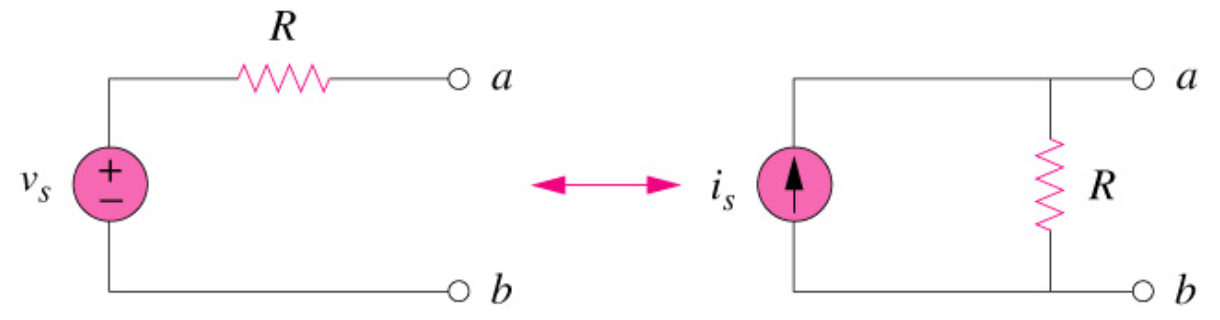
\includegraphics[width=20em]{images/source_transform.png}
\end{center}
\[V=IR\]

\heading{Thevenin}
\begin{enumerate}[topsep=0pt,noitemsep]
    \item $V_{th}=V_{oc}$, turn off independent sources to get $R_{th}$
    \item $V_{th}=V_{oc}$, find $I_{sc}$ then $R_{th}=V_{oc}/I_{sc}$
    \item Apply test current/test voltage
    \item Source transform
\end{enumerate}

\heading{Norton}
\[I_n=V_{th}/R_{th}\qquad R_n=R_{th}\]

\heading{Maximum Power}
\[R_L=R_{th}\qquad P_{max}=\frac{V^2}{4R_{th}}\]

\sectionheading{Capacitors and Inductors}
\heading{Capacitors}
\[q=CV \qquad i=C\dv vt \qquad W=\frac 12 Cv^2\]

\heading{Inductors}
\[v=L\dv it \qquad W=\frac 12Li^2\]

\sectionheading{First/Second Order Circuits}
\textbf{First Order}
\[\tau=RC \qquad \tau=\frac LR\tag{use $R=R_{th}$}\]
\[x(t)=\sqb{x(t_0^+)-x(\infty)}e^{-\frac{t-t_0}{\tau}}+x(\infty)\]
\textbf{Second Order}

Solve second order constant coefficient DE. 

\sectionheading{OpAmps}

\begin{itemize}[topsep=0pt,noitemsep]
    \item Saturate at $+V_{cc}$ and $-V_{cc}$
    \item Amplifier: $V_{out}=AV_{in}$
    \item Negative feedback: $i_+=i_-=0\qquad V_+=V_-$
\end{itemize}
\begin{center}
    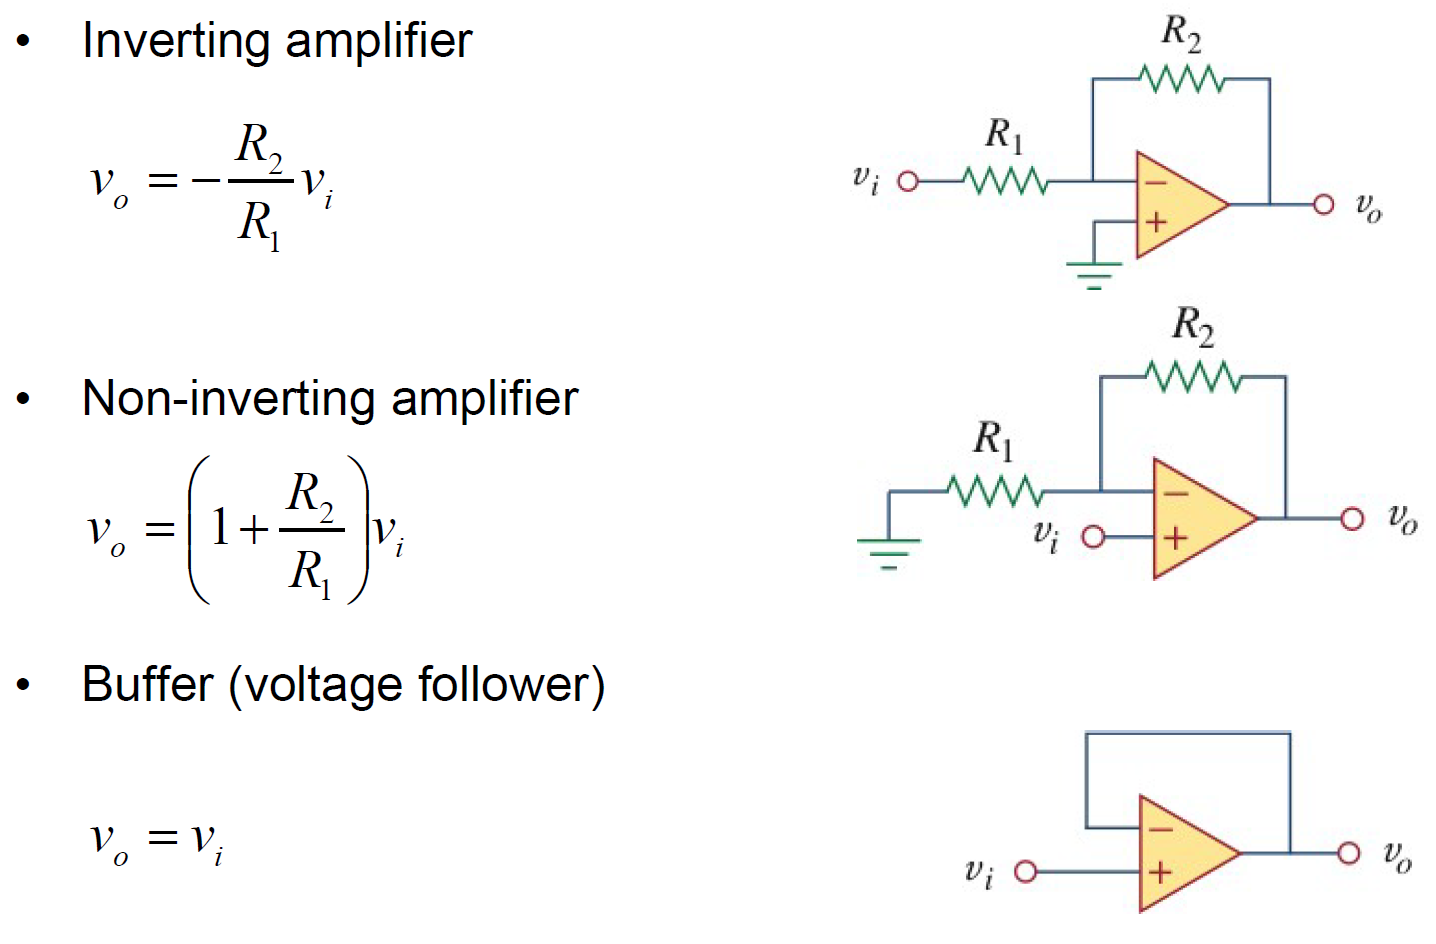
\includegraphics[width=20em]{images/opamp_1.png}
    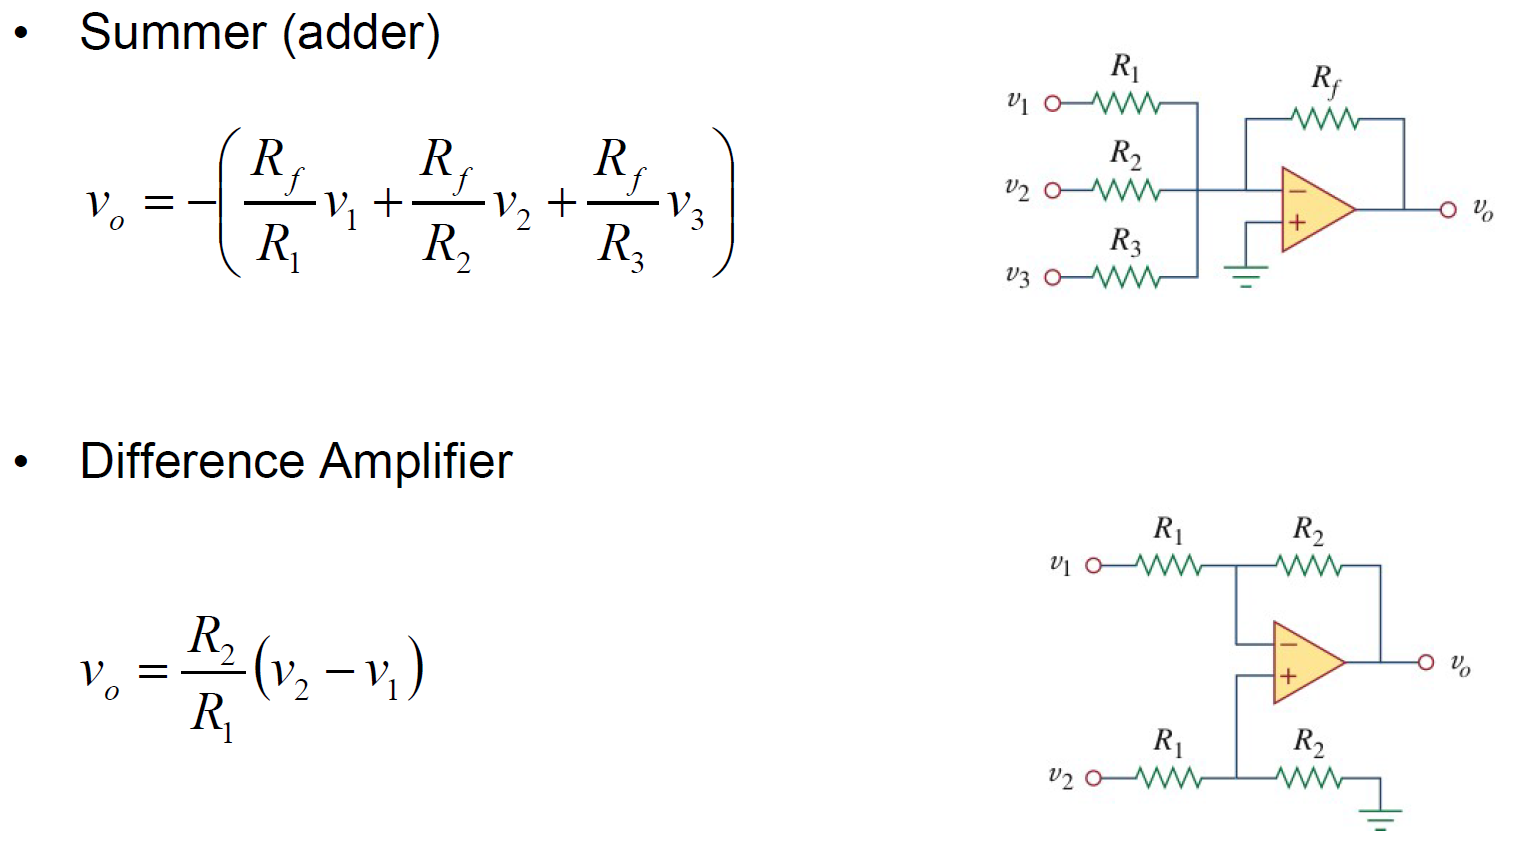
\includegraphics[width=20em]{images/opamp_2.png}
    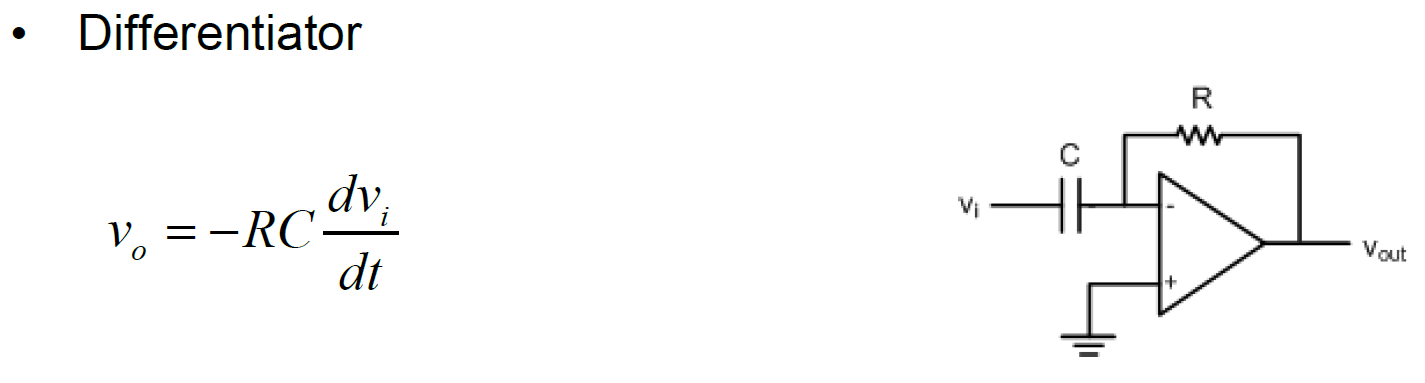
\includegraphics[width=20em]{images/opamp_3.png}
    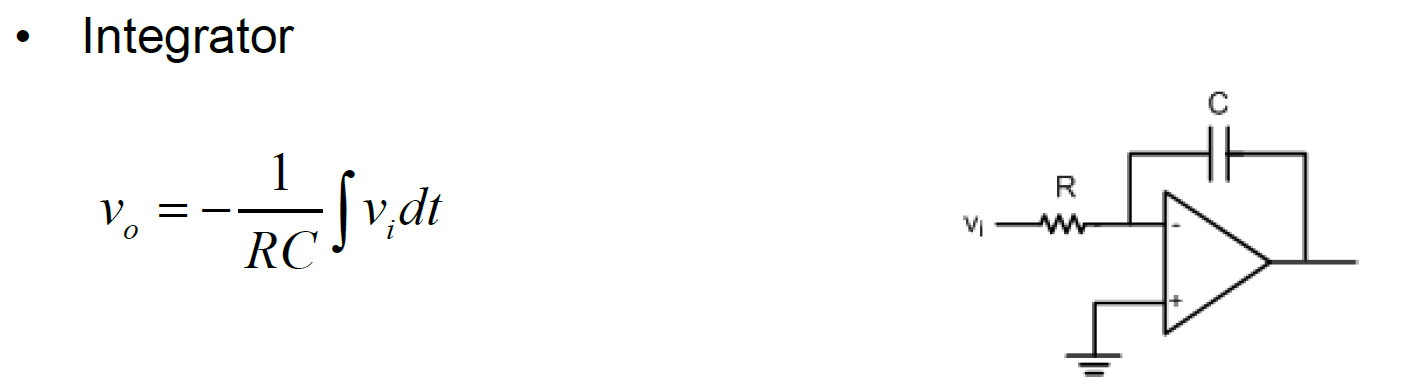
\includegraphics[width=20em]{images/opamp_4.png}
    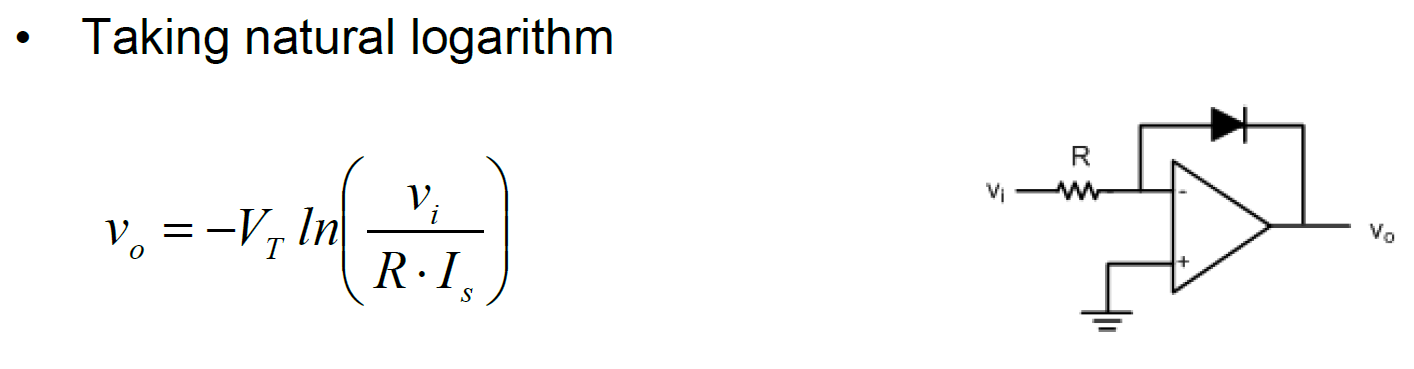
\includegraphics[width=20em]{images/opamp_5.png}
    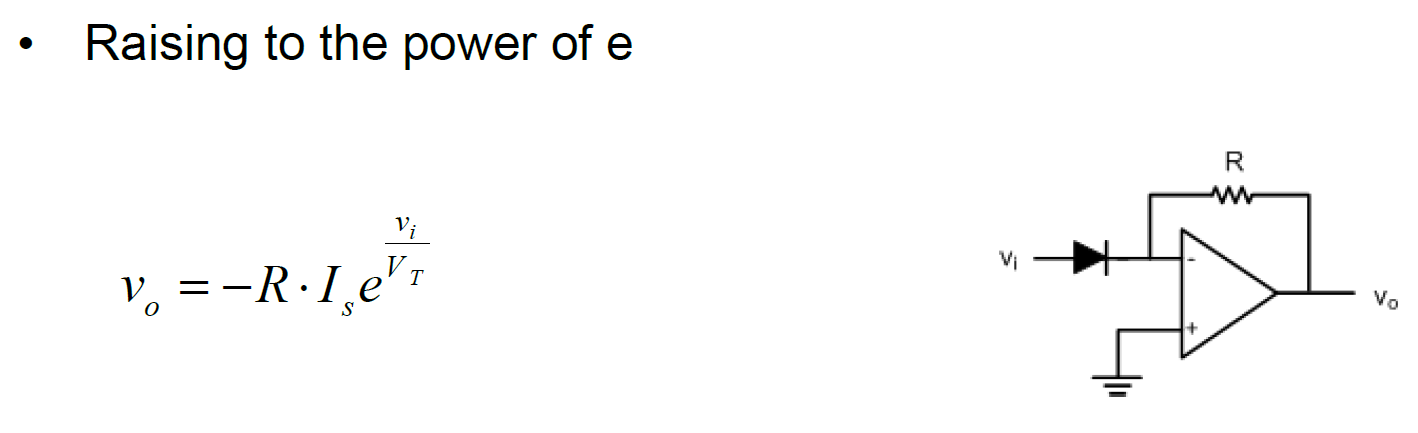
\includegraphics[width=20em]{images/opamp_6.png}
\end{center}

\sectionheading{Sinusoidal Analysis and Power}
\heading{Sinusoidal Analysis}
\[v(t)=V_m\cos(\omega t+\theta)=\Re{V_me^{j\theta}e^{j\omega t}}\]
\[v(t)\equiv\Re{V_me^{j\theta}}=\Re{V_m\phase\theta}=\Re{\V}\]
\[\Z=R+jX\]
\[X_L=\omega L \qquad X_C=-\frac{1}{\omega C}\]
\begin{itemize}[topsep=0pt,noitemsep]
    \item $\V,\I,\Z$ can be treated as $V,I,R$.
    \item Thevenin, Nodal, and Mesh analysis $\checkmark$
\end{itemize}

\heading{Real Power}
\begin{align*}
    p&=\underbrace{\frac{V_mI_m}{2}\cos(\theta_v-\theta_i)}_{P:\text{ active power}}+\frac{V_mI_m}{2}\cos(\theta_v-\theta_i)\cos 2\omega t \\
    &\hspace{1em}-\underbrace{\frac{V_mI_m}{2}\sin(\theta_v-\theta_i)}_{Q:\text{ reactive power}} \sin 2\omega t
\end{align*}

Power factor: $pf=\cos(\theta_v-\theta_i)$.

RMS:
\[I_{rms}=I_{eff}=\frac{I}{\sqrt 2} \qquad V_{rms}=V_{eff}=\frac{V}{\sqrt 2}\]

\heading{Complex Power}
\[\S=P+jQ=\V_{rms}\I\conj_{rms}=\frac 12\V\I\conj\]
\[\S=\Z\I_{eff}\I\conj_{eff}=\Z\norm{\I_{eff}}^2\]
\[P=\norm{\I_{eff}}^2R=\frac 12\norm{\I}^2R\]
\[Q=\norm{\I_{eff}}^2X=\frac 12\norm{\I}^2X\]

\heading{Maximum Power}

\[\Z_L=\Z\conj_{th} \qquad P_{max}=\frac 14\frac{\norm{\V_{th}}^2}{R_{th}}\]

Restricted $R_L$ and $X_L$:
\begin{itemize}[topsep=0pt,noitemsep]
    \item Adjust $X_L$ to be close to $-X_{th}$
    \item Adjust $R_L$ to be close to $\sqrt{R_{th}^2+(X_L+X_{th})^2}$
\end{itemize}
Fixed angle of $\Z_L$:
\begin{itemize}[topsep=0pt,noitemsep]
    \item Set $\norm{\Z_L}=\norm{\Z_{th}}$
\end{itemize}

\heading{Diodes}

\[i_D=I_0\lrb{e^{\frac{v_D}{nV_T}}-1} \qquad V_T\equiv\frac{kT}{q_e}\]
\[V_D=\SI{0.7}{\volt}\]

\begin{enumerate}[topsep=0pt,noitemsep]
    \item Assume whether each diode is on or off, solve for currents/voltage, and check if consistent with assumption
    \item If inconsistent, try another combination
\end{enumerate}

\heading{BJTs - NPN}

Linear zone: BE forward biased and BC reverse biased

\begin{center}
    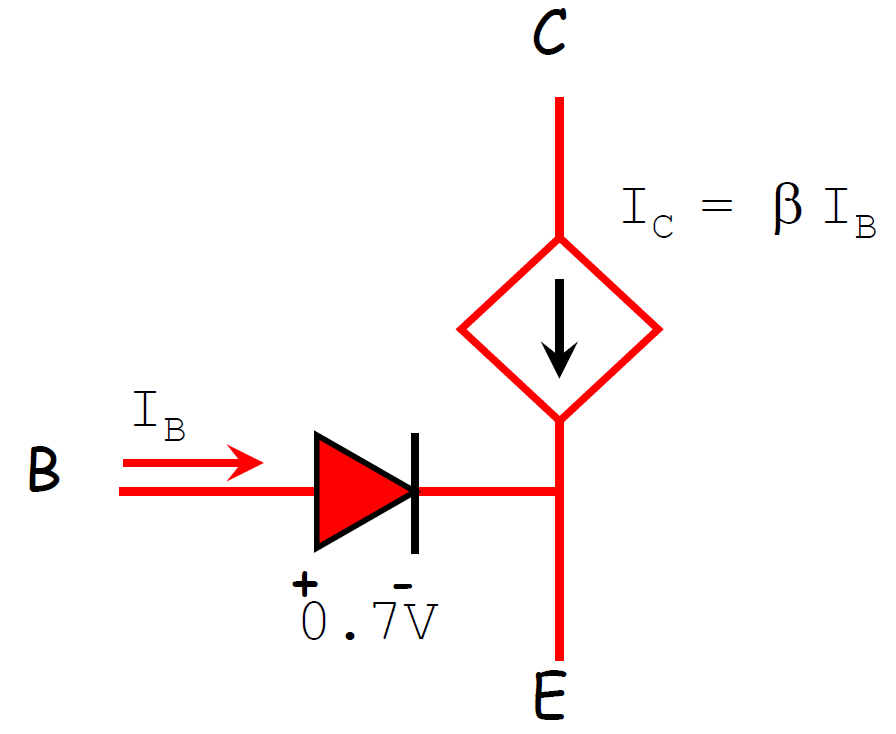
\includegraphics[width=8em]{images/bjt_diode.png} 
\end{center}

\begin{enumerate}[topsep=0pt,noitemsep]
    \item DC operating point: turn off AC sources, solve
    \item AC small-signal: turn off DC sources, use hybrid-pi small signal equivalent
\end{enumerate}

\[g_m=\frac{I_C}{V_T} \qquad r_\pi = \frac{\beta}{g_m}=\frac{\beta V_T}{I_C}=\frac{V_T}{I_B}\]

\begin{center}
    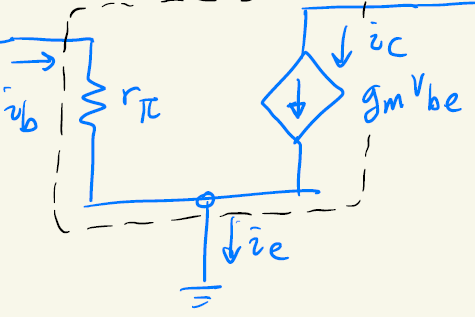
\includegraphics[width=10em]{images/bjt_hybrid_pi.png}
\end{center}

\heading{MOSFETs - NMOS}

Activate when $V_{GS}>V_{Th}$

\begin{itemize}[topsep=0pt,noitemsep]
    \item $V_{DS}\ll V_{GS}-V_{Th}$ (deep triode):
    \[I_D=\mu_nC_{ox}\frac WL(V_{GS}-V_{Th})\cdot V_{DS}\]
    \item $V_{DS}\le V_{GS}-V_{Th}$ (triode):
    \[I_D=\mu_nC_{ox}\frac WL\sqb{(V_{GS}-V_{Th})\cdot V_{DS}-\frac 12V_{DS}^2}\]
    \[g_m=\mu_nC_{ox}\frac WLV_{DS}\]
    \item $V_{DS}>V_{GS}-V_{Th}$ (saturation):
    \[I_D=\frac 12\mu_nC_{ox}\frac WL(V_{GS}-V_{Th})^2\]
    \[g_m=\mu_nC_{ox}\frac WL(V_{GS}-V_{Th})\]
\end{itemize}

\newcolumn
Small signal equivalent:

\begin{center}
    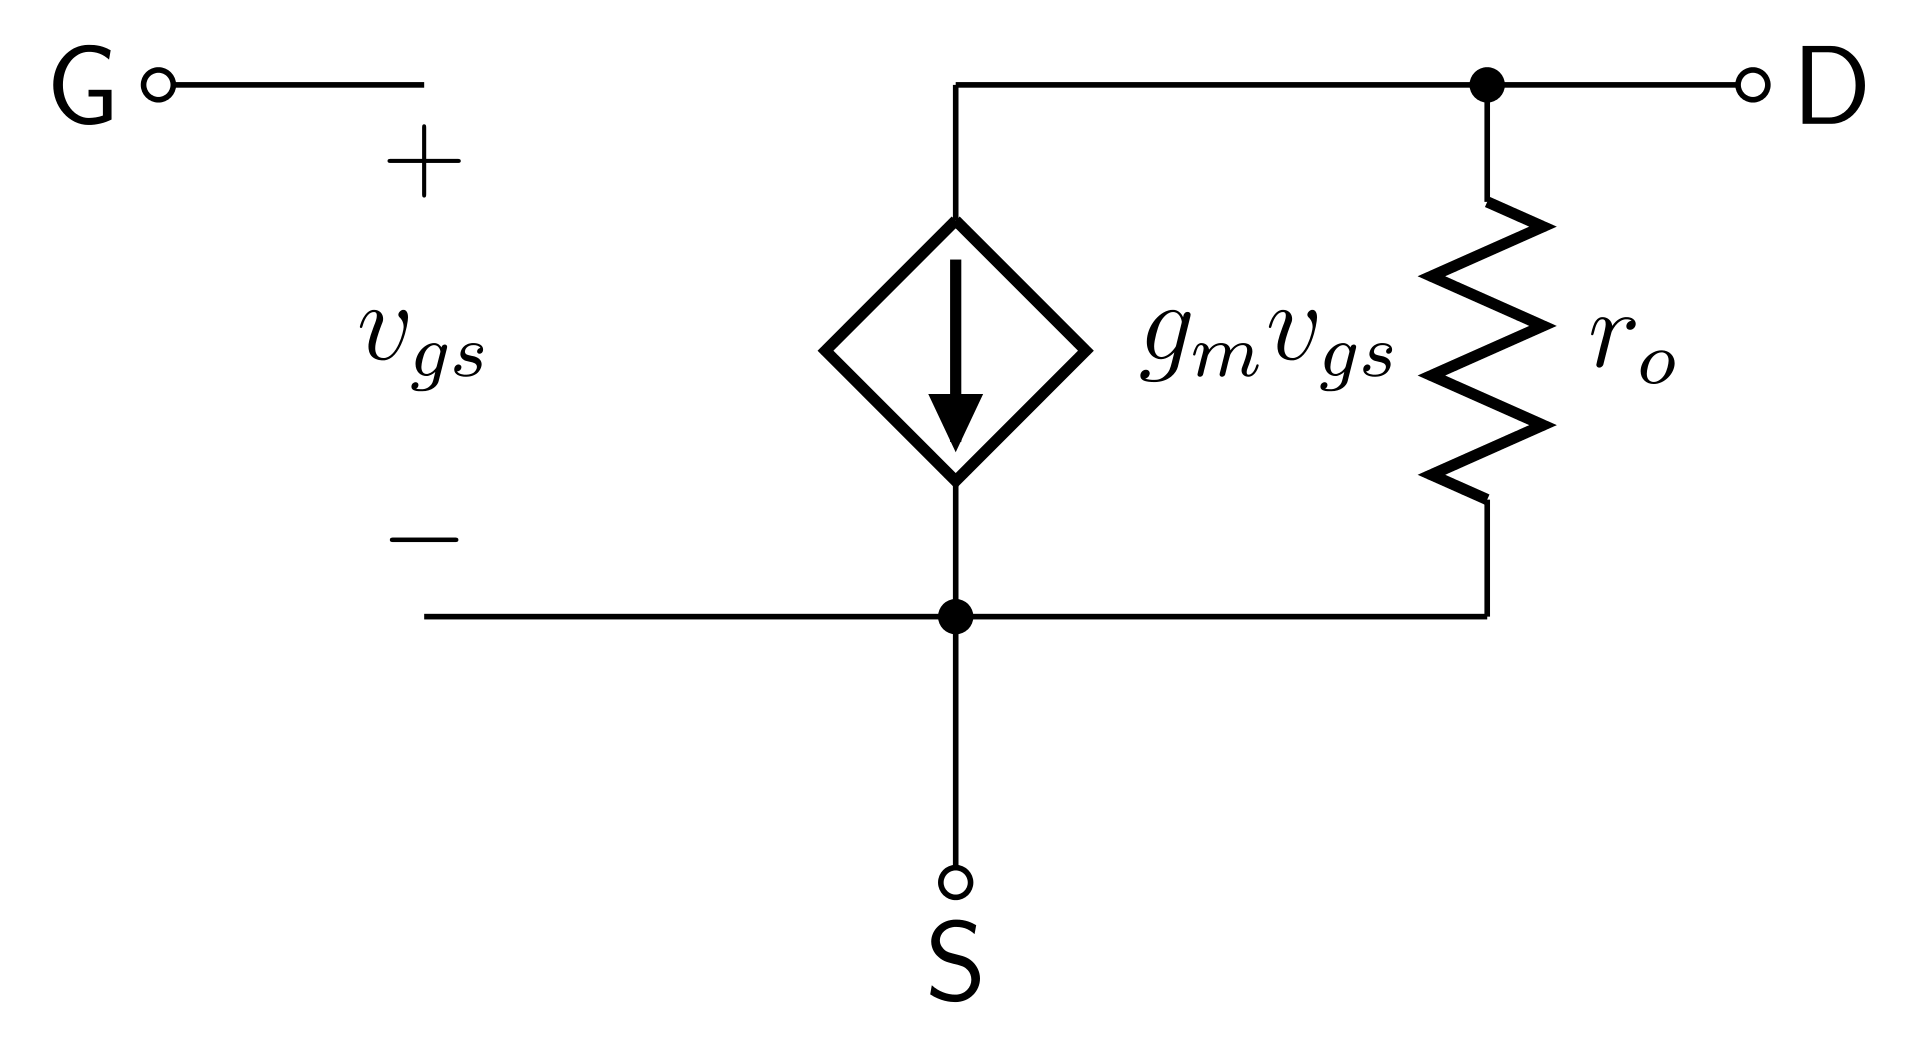
\includegraphics[width=10em]{images/mosfet_hybrid_pi.png} 
\end{center}

\end{multicols*}


\end{document}